%\input{Preambulum}

\begin{figure}[t!]
\centering

\begin{subfigure}{\textwidth}
\caption{Graphs with pair constraints ($G_1$--$G_{31}$ plus two pairs of nodes, Figure~\ref{Fig1})}
\label{Fig7a}

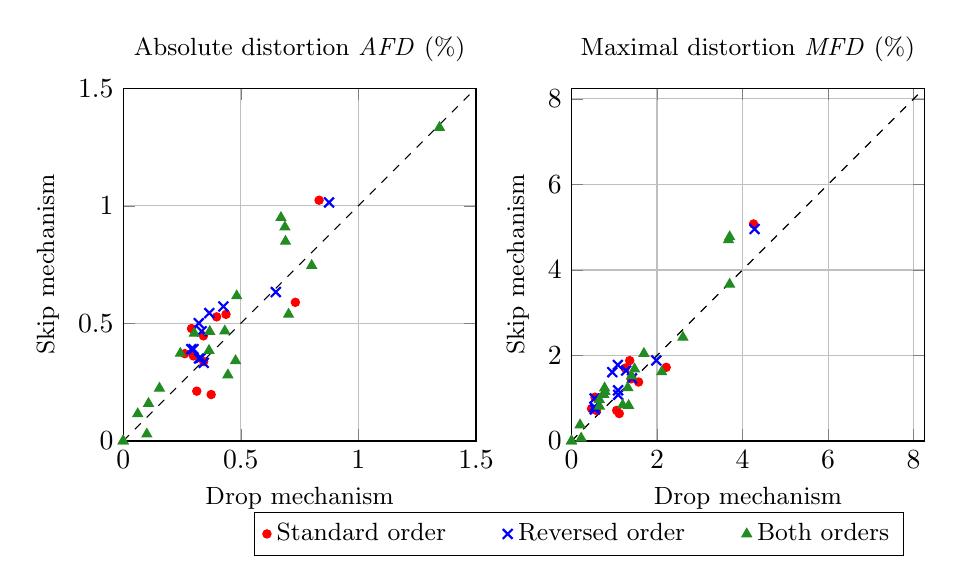
\begin{tikzpicture}
\begin{axis}[
name = axis1,
title = {Absolute distortion $\mathit{AFD}$ (\%)},
title style = {font=\small},
xlabel = Drop mechanism,
x label style = {font=\small},
ylabel = Skip mechanism,
y label style = {font=\small},
width = 0.5\textwidth,
height = 0.5\textwidth,
nodes near coords,
xmajorgrids = true,
ymajorgrids = true,
xmin = 0,
xmax = 1.5,
ymin = 0,
ymax = 1.5,
]
\addplot [scatter,red,only marks,mark size=1.5pt,point meta=explicit symbolic] coordinates {
(0.298701946274677,0.361866077667965)
(0.342065125089788,0.337595532039976)
(0.397361201644333,0.527814209223831)
(0.261620751409832,0.371456332876086)
(0.437208912317014,0.538539930835528)
(0.341191104929326,0.447137782436524)
(0.29047247578992,0.478068007829912)
(0.832881407259646,1.02368560253125)
(0.312910012854697,0.211921215415276)
(0.374111099805549,0.197564780898114)
(0.731993395725481,0.589673436877738)
};
\addplot [scatter,blue,only marks,mark=x,mark size=2.5pt,thick,point meta=explicit symbolic] coordinates {
(0.298704702006573,0.390305231107118)
(0.330551064733154,0.35371350186165)
(0.366202314800251,0.543789289242121)
(0.289396623990251,0.390775034293552)
(0.426135914831561,0.571837651633249)
(0.333679827626382,0.466724677023419)
(0.321499473483577,0.500860030621936)
(0.875307132196234,1.01431715389394)
(0.322723684551085,0.351153039832286)
(0.342214138741933,0.332417582417582)
(0.649035576795451,0.633191955396256)
};
\addplot [scatter,ForestGreen,only marks,mark=triangle*,mark size=2pt,point meta=explicit symbolic] coordinates {
(0,0)
(0.107650786765948,0.159630352538616)
(0,0)
(0.154251608050623,0.224396008403362)
(0.302345807506964,0.458098857183636)
(0.367949817101051,0.465477823502515)
(0.100520348342374,0.0293697996455505)
(0.243111292858728,0.372543734559678)
(0.0618727195481796,0.115659519168292)
(0.432026175895945,0.46743295019157)
(0.801469782955018,0.746059645253194)
(0.364873088689801,0.384741902834007)
(0.670770227049451,0.949757512055246)
(0.690035579561043,0.848641975308641)
(0.687544165196933,0.909497354497355)
(0.477750079138961,0.341405508072174)
(0.482694911502165,0.617019071310116)
(0.445166338772197,0.28091157678146)
(1.34462129714655,1.33287419651056)
(0.703076774691382,0.538580246913581)
};
% Zero line
\draw [black,dashed] (rel axis cs:0,0) -- (rel axis cs:1,1);
\end{axis}

\begin{axis}[
at = {(axis1.south east)},
xshift = 0.1\textwidth,
title = {Maximal distortion $\mathit{MFD}$ (\%)},
title style = {font=\small},
xlabel = Drop mechanism,
x label style = {font=\small},
ylabel = Skip mechanism,
y label style = {font=\small},
width = 0.5\textwidth,
height = 0.5\textwidth,
nodes near coords,
xmajorgrids = true,
ymajorgrids = true,
xmin = 0,
xmax = 8.25,
ymin = 0,
ymax = 8.25,
legend style = {font=\small,at={(-0.9,-0.2)},anchor=north west,legend columns=3},
legend entries = {Standard order$\qquad$,Reversed order$\qquad$,Both orders}
]
\addplot [scatter,red,only marks,mark size=1.5pt,point meta=explicit symbolic] coordinates {
(0.580902231830868,0.714033018867924)
(1.56851851851843,1.37962962962963)
(1.36085091532357,1.88008316841014)
(0.467923739711942,0.755401234567901)
(1.39564455703091,1.45384928954111)
(1.25767856102952,1.70619322152341)
(0.550228594524232,1.02535273368606)
(4.25643966599363,5.07544258094572)
(1.05607129338458,0.715234102026555)
(1.11729772927691,0.642085537918871)
(2.21436720098232,1.72253335324571)
};
\addplot [scatter,blue,only marks,mark=x,mark size=2.5pt,thick,point meta=explicit symbolic] coordinates {
(0.545785290006939,0.73833857442348)
(1.41296296296292,1.46527777777778)
(1.08409551408905,1.77900292149656)
(0.536731610082294,0.799768518518518)
(1.27695242740119,1.6498369438621)
(0.95313252193493,1.60974260423946)
(0.54203672209629,0.995260141093474)
(4.28125533814724,4.95661542045189)
(1.08919243535988,1.18514150943396)
(1.09261923133452,1.08035714285714)
(1.98221378020048,1.88457039028275)
};
\addplot [scatter,ForestGreen,only marks,mark=triangle*,mark size=2pt,point meta=explicit symbolic] coordinates {
(0,0)
(0.780468204053092,1.15732005590496)
(0,0)
(0.651308324255606,0.814406318082789)
(0.773765599354204,1.23889870120602)
(0.754019694297536,1.08553791887125)
(0.226170783770452,0.0660820492024872)
(0.651640053697788,0.964625521804779)
(0.20108633853152,0.375893437296945)
(1.40408507166182,1.51915708812261)
(2.6047767946038,2.42469384707288)
(1.47520796106778,1.68433235867446)
(3.69871037096964,4.77421191417955)
(1.69331490054872,2.0462962962963)
(3.66999559082877,4.70271164021164)
(1.19652777777783,0.840277777777779)
(1.31653972933688,1.24675234936429)
(1.33549901631655,0.829536224821312)
(3.697708567153,3.66540404040404)
(2.10923032407412,1.61574074074074)
};
% Zero line
\draw [black,dashed] (rel axis cs:0,0) -- (rel axis cs:1,1);
\end{axis}
\end{tikzpicture}
\end{subfigure}

\vspace{0.25cm}
\begin{subfigure}{\textwidth}
\caption{Graphs without pair constraints ($H_1$--$H_{31}$ plus two pairs of nodes, Figure~\ref{Fig2})}
\label{Fig7b}

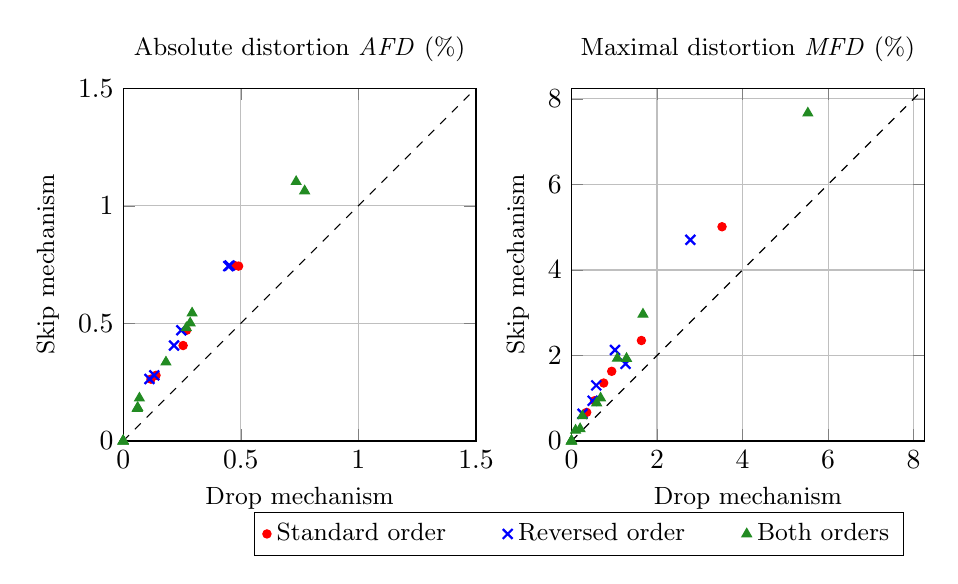
\begin{tikzpicture}
\begin{axis}[
name = axis1,
title = {Absolute distortion $\mathit{AFD}$ (\%)},
title style = {font=\small},
xlabel = Drop mechanism,
x label style = {font=\small},
ylabel = Skip mechanism,
y label style = {font=\small},
width = 0.5\textwidth,
height = 0.5\textwidth,
nodes near coords,
xmajorgrids = true,
ymajorgrids = true,
xmin = 0,
xmax = 1.5,
ymin = 0,
ymax = 1.5,
]
\addplot [scatter,red,only marks,mark size=1.5pt,point meta=explicit symbolic] coordinates {
(0.139644814154627,0.279263220439691)
(0.118137039697745,0.263150542784163)
(0.269356261022915,0.47089947089947)
(0.474759945130307,0.745679012345679)
(0.254825498575496,0.405982905982905)
(0.490697295536005,0.74356467904855)
};
\addplot [scatter,blue,only marks,mark=x,mark size=2.5pt,thick,point meta=explicit symbolic] coordinates {
(0.132237406747227,0.279263220439691)
(0.111713428586646,0.263729246487866)
(0.247134038800716,0.47089947089947)
(0.452674897119323,0.74567901234568)
(0.216168091168065,0.405982905982905)
(0.446790485500152,0.74356467904855)
};
\addplot [scatter,ForestGreen,only marks,mark=triangle*,mark size=2pt,point meta=explicit symbolic] coordinates {
(0,0)
(0,0)
(0.0597572362278245,0.138188608776844)
(0.069042538056659,0.182173851187936)
(0.0618727195481796,0.142201248209536)
(0,0)
(0.29295634920635,0.543650793650794)
(0.181831054471436,0.335324571883711)
(0,0)
(0.268646526711035,0.481310803891449)
(0.284832481190496,0.501533857089412)
(0.735336283094566,1.10257124292212)
(0,0)
(0.771574074074071,1.06296296296296)
};
% Zero line
\draw [black,dashed] (rel axis cs:0,0) -- (rel axis cs:1,1);
\end{axis}

\begin{axis}[
at = {(axis1.south east)},
xshift = 0.1\textwidth,
title = {Maximal distortion $\mathit{MFD}$ (\%)},
title style = {font=\small},
xlabel = Drop mechanism,
x label style = {font=\small},
ylabel = Skip mechanism,
y label style = {font=\small},
width = 0.5\textwidth,
height = 0.5\textwidth,
nodes near coords,
xmajorgrids = true,
ymajorgrids = true,
xmin = 0,
xmax = 8.25,
ymin = 0,
ymax = 8.25,
legend style = {font=\small,at={(-0.9,-0.2)},anchor=north west,legend columns=3},
legend entries = {Standard order$\qquad$,Reversed order$\qquad$,Both orders}
]
\addplot [scatter,red,only marks,mark size=1.5pt,point meta=explicit symbolic] coordinates {
(0.752505446623097,1.3562091503268)
(0.355034057045608,0.669540229885057)
(0.53871252204587,0.941798941798944)
(0.939943415637956,1.62962962962963)
(1.63468660968671,2.35042735042735)
(3.51982323232322,5.01010101010101)
};
\addplot [scatter,blue,only marks,mark=x,mark size=2.5pt,thick,point meta=explicit symbolic] coordinates {
(0.578431372549021,1.30065359477124)
(0.257503192848008,0.637132822477648)
(0.49426807760152,0.941798941798944)
(1.26311728395064,1.80555555555556)
(1.01709401709393,2.12820512820513)
(2.77954545454538,4.70454545454546)
};
\addplot [scatter,ForestGreen,only marks,mark=triangle*,mark size=2pt,point meta=explicit symbolic] coordinates {
(0,0)
(0,0)
(0.253968253968254,0.587301587301586)
(0.0949334898278864,0.250489045383412)
(0.20108633853152,0.28440249641907)
(0,0)
(1.6712301587302,2.96428571428571)
(1.07268518518517,1.93209876543209)
(0,0)
(0.680224867724932,1.00198412698412)
(0.588566997131759,0.889450056116722)
(1.28683849541548,1.92949967511371)
(0,0)
(5.52638888888876,7.66666666666667)
};
% Zero line
\draw [black,dashed] (rel axis cs:0,0) -- (rel axis cs:1,1);
\end{axis}
\end{tikzpicture}
\end{subfigure}

\caption{Fairness distortions of the draw mechanisms \\ for selected balanced bipartite graphs with 12 nodes ($n=6$)}
\label{Fig7}
\end{figure}

%\end{document}